\documentclass[a4paper,11pt]{report}

% Packages for document formatting
\usepackage[utf8]{inputenc} % UTF-8 encoding
\usepackage[T1]{fontenc}   % Font encoding
\usepackage{lmodern}       % Improved fonts
\usepackage{geometry}      % Page layout
\geometry{a4paper, margin=1.5in}
\usepackage{setspace}      % Line spacing
\setstretch{1.2}
\usepackage{titlesec}      % Customizable section titles
\titleformat{\chapter}[display]
  {\normalfont\huge\bfseries}{\chaptername\ \thechapter}{20pt}{\Huge}

% Bibliography management
\usepackage[backend=biber,style=nature]{biblatex} % APA style, customizable
\addbibresource{ref.bib} % Bibliography file

% Acronyms
\usepackage[acronym,nonumberlist]{glossaries}
\makeglossaries

% Hyperlinks
\usepackage{hyperref}
\hypersetup{
    colorlinks=true,
    linkcolor=black,
    citecolor=teal,
    filecolor=magenta,
    urlcolor=cyan
}
\usepackage{cleveref} % Smart referencing

% Graphics and tables
\usepackage{graphicx}       % Include images
\usepackage{float}          % Improved figure placement
\usepackage{caption}        % Customizable captions
\usepackage{subcaption}     % Subfigures
\usepackage{booktabs}       % Improved tables
\usepackage{longtable}      % Tables spanning multiple pages

% Math and algorithms
\usepackage{amsmath,amssymb,amsfonts} % Math symbols and fonts
\usepackage{amsthm}          % Theorem environments
\usepackage{mathtools}      % Additional math tools
\usepackage{algorithm}
\usepackage{algpseudocode}

\theoremstyle{definition}
\newtheorem{definition}{Definition}[section]
\theoremstyle{plain}


% Code formatting
\usepackage{listings}       % Include code
\usepackage{xcolor}         % Colors for listings
\lstset{
    basicstyle=\ttfamily\small,
    keywordstyle=\color{blue},
    commentstyle=\color{gray},
    stringstyle=\color{red},
    numbers=left,
    numberstyle=\tiny\color{gray},
    breaklines=true,
    frame=single
}

% Document metadata
\title{\textbf{Reinforcement Learning for Robotic Surgery}}
\author{Matteo Nunziante}
\date{\today}

\begin{document}

% Title page
\maketitle

% Abstract
\chapter*{Abstract}
\addcontentsline{toc}{chapter}{Abstract}
Your abstract here...

% Acknowledgments
\chapter*{Acknowledgments}
\addcontentsline{toc}{chapter}{Acknowledgments}
Your acknowledgments here...

% Table of Contents
\tableofcontents
\listoffigures
\listoftables

% Acronyms
\addcontentsline{toc}{chapter}{Acronyms}
\printglossary[type=\acronymtype]
\newacronym{rl}{RL}{Reinforcement Learning}
\newacronym{mdp}{MDP}{Markov Decision Process}
\newacronym{pomdp}{POMDP}{Partially Observable Markov Decision Process}
\newacronym{llm}{LLM}{Large Language Model}

% Chapters
\chapter{Introduction}
Introduction content here...

\chapter{Reinforcement Learning}
\section{Overview}

\gls{rl} is a subfield of machine learning focused on the problem of learning 
optimal behaviors: an agent repeatedly interacts with an environment, balancing 
exploration (trying new actions) and exploitation (using known strategies) 
to maximize a reward. \

For instance, consider a baby learning to walk: it repeatedly attempts to stand 
and take steps, getting positive feedback for each successful movement and 
negative feedback from falls. Over time, it refines its attempts to walk 
more effectively. \

Differently from supervised learning, where the agent is trained on labeled data, 
and from unsupervised learning, where the agent must find patterns in unlabeled data,
\gls{rl} makes use of rewards and punishments, making it suitable for problems 
where the agent (be it a baby or a \gls{llm}) must learn through trial and error, creating its own training data 
through interaction.

% quclosa circa policy e value 
% The concepts of value and value function are key to most of the reinforcement learning
% methods that we consider in this book. We take the position that value functions
% are important for efficient search in the space of policies. The use of value functions
% distinguishes reinforcement learning methods from evolutionary methods that search
% directly in policy space guided by evaluations of entire policies.

% related formal example 
% 
% 
% 
% 

% online vs offline learning
% 
% 
% 
% 
% 

In the next sections, we will introduce the foundational concepts of \gls{rl}, 
mathematical frameworks, and algorithms that enable agents to learn optimal behaviors for 
a wide range of tasks.


\section{Markov Decision Process}
\begin{figure}
    \centering
    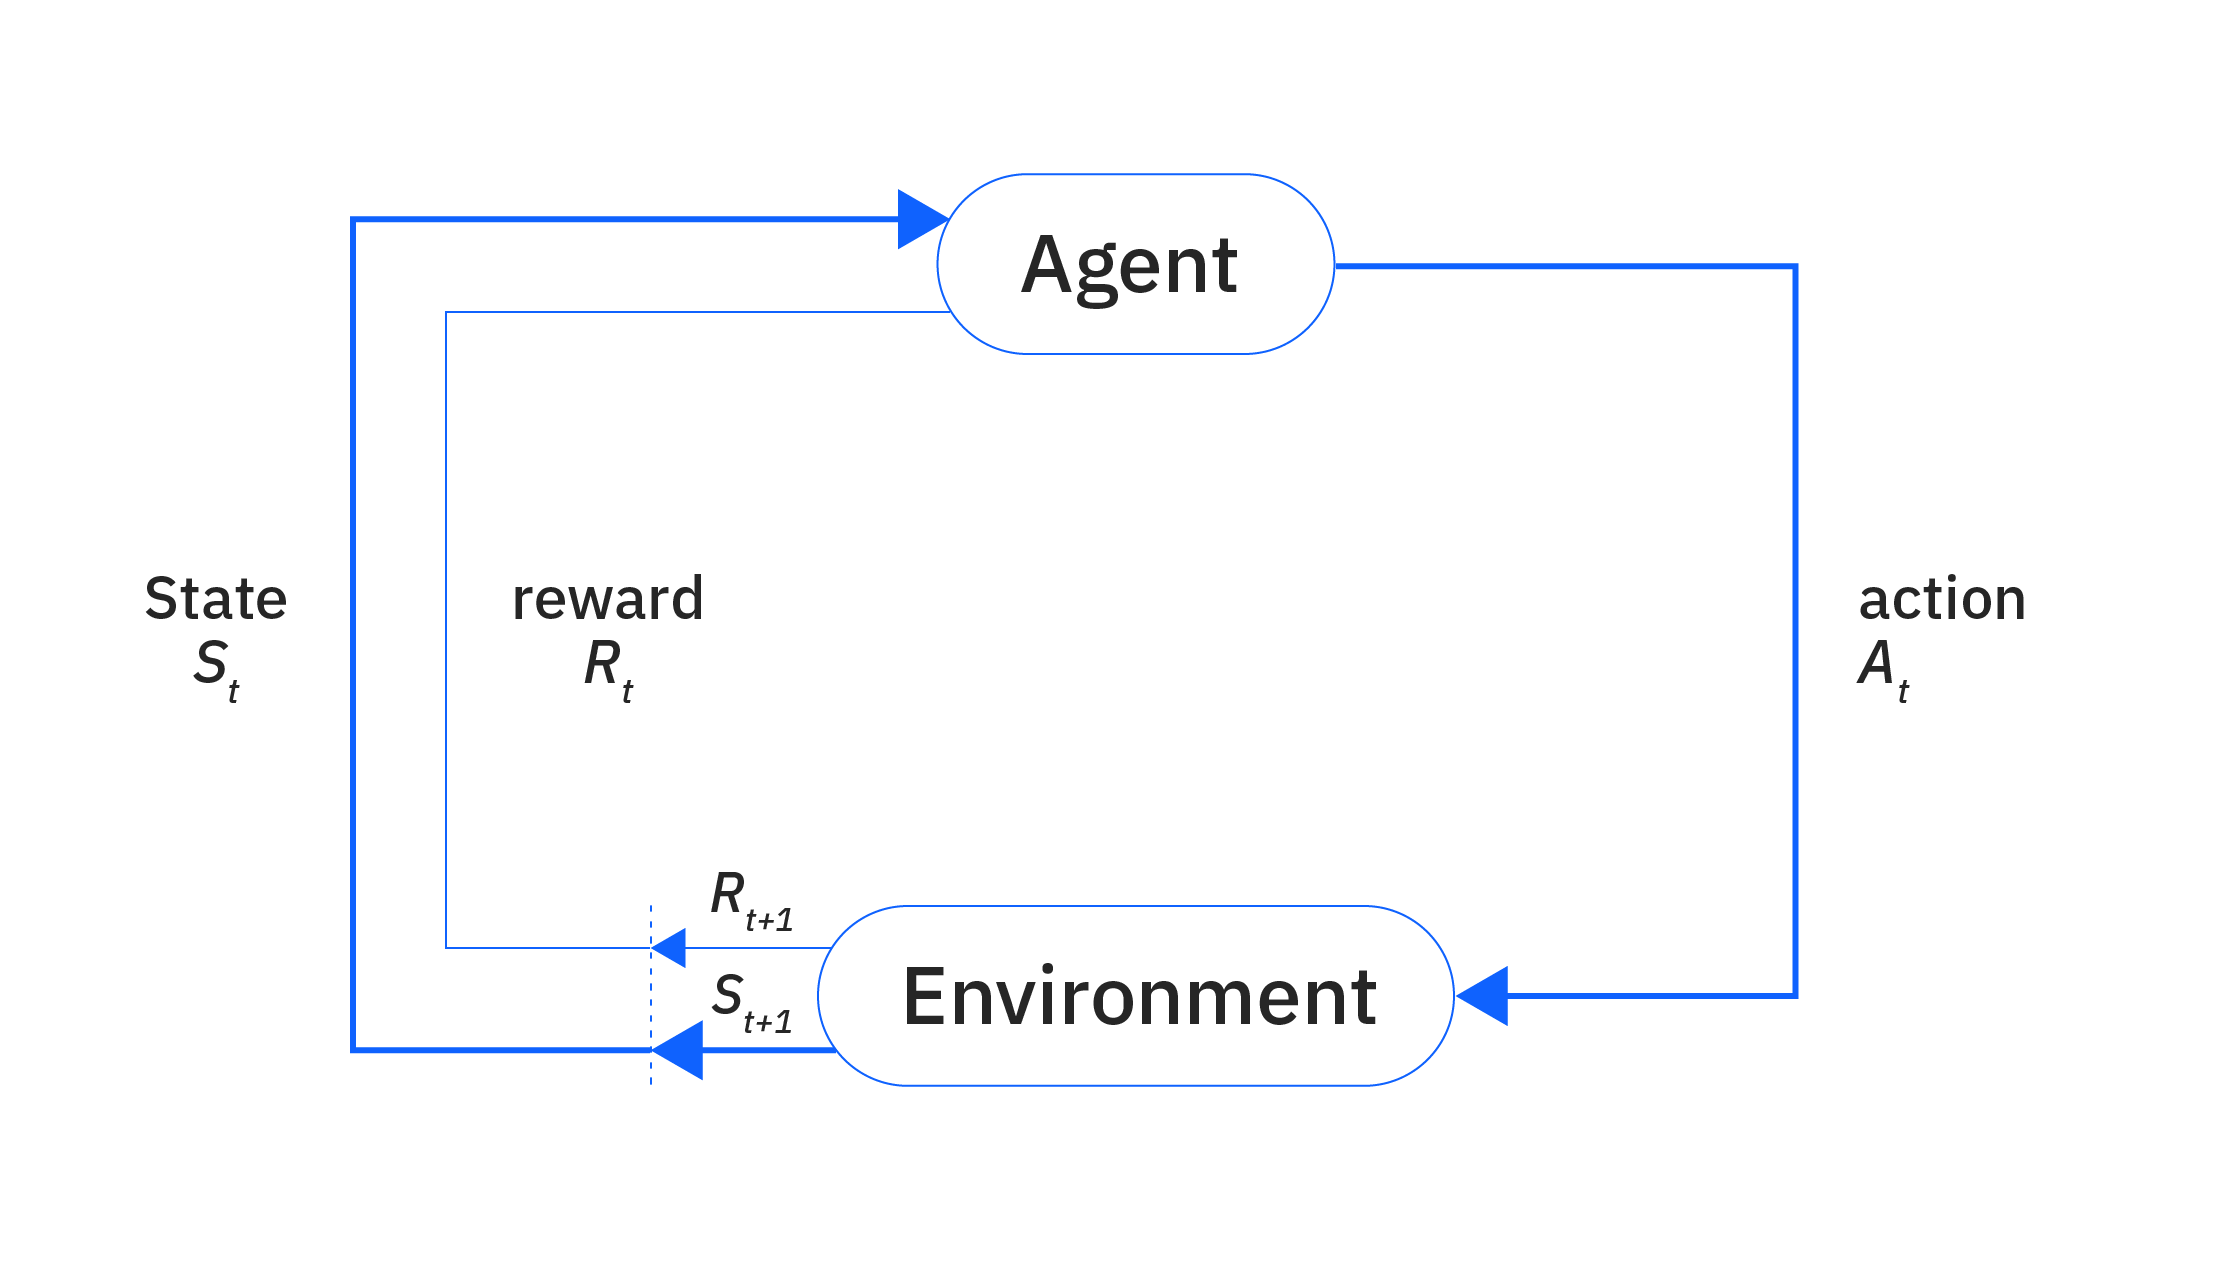
\includegraphics[width=0.5\textwidth]{images/MDP.png}
    \caption{Markov Decision Process}
    \label{fig:mdp}
\end{figure}

Reinforcement learning leverages \gls{mdp}s to model interactions between 
an agent and its environment in terms of states, actions, and rewards. 
This framework captures in a simple way features of the problem such as cause-and-effect, 
uncertainty, and explicit objectives.
Although general \gls{mdp}s may have infinite (even uncountable) state and action
spaces, we limit the discussion to finite-state and finite-action problems.
naturally occur.
A \gls{mdp} is a model for sequential decision making in a probabilistic environment, it requires
the following components:

\subsection*{States}
The set of environmental states $S$ is defined as the finite set $\{s_1 , . . . , s_N \}$ where the
size of the state space is $|S| = N$. A state is a unique characterization of all
that is important (at given time) of the problem that is modelled. For example, a chess game state 
could be the position of all the pieces on the board.

\subsection*{Actions}
The set of actions A is defined as the finite set $\{a_1 , . . . , a_K \}$ where the size of the
action space is $|A| = K.$. Actions can be used to control the system state.
The set of actions that can be applied in some particular state $s \in S$, is denoted $A(s)$,
where $A(s) \subset A$. In some systems, not all actions can be applied in every state, but in
general we will assume that $A(s) = A$ for all $s \in S$.

\subsection*{Trasition Function}
By applying action $a \in A$ in a state $s \in S$, the system makes a transition from s to a
new state $s' \in S$, based on a probability distribution over the set of possible transitions. 
The transition function T is defined as 
$$T : S \times A \times S \rightarrow [0,1]$$ which represents the probability
of ending up in state s' after doing action a in state s is denoted $ T(s,a,s')$. It is required that 
for all actions a, and all states s and s', $T (s,a,s') \geq 0$ and for all states s and actions a, 
$$\sum_{s' \in S} T (s,a,s') = 1$$
such that T defines a proper probability distribution over possible next states. \

The sequential nature of the framework is captured by that of \textit{Markov chain}:
a Markovian Stochastic Process. 
Stochastic Processes araise in many problems from the natural sciences
in which one has to keep track of a value observed at time t. 

The process is Markovian if the result of an action does not
depend on the previous actions and history of visited states, but only depends on the
current state.

Going back to our notation, given a trajectory of the form 
$$s_0, a_0, . . . . , s_t, a_t, s_{t+1}$$
the Markov property is defined as follows:

$$P(s_{t+1} | s_t ,a_t ,s_{t_1} ,a_{t-1} , . . ,s_0,a_0) = P(s_{t+1} | s_t ,a_t ) = T (s_t ,a_t ,s_{t+1} )$$

The idea of Markovian dynamics is that the current state s gives enough information
to make an optimal decision; it is not important which states and actions preceded s.

\subsection*{Reward Function}
Rewards guide learning by signaling success. A higher reward indicates a more 
desirable outcome. In the maze example, reaching the exit might give a large positive 
reward, encouraging the agent to repeat the actions that led to that success.


With the above components, we can define a \gls{mdp}.

\begin{definition}
A Markov Decision Process \gls{mdp} is a tuple $M = (S, A, T, R)$ where:
\begin{itemize}
    \setlength\itemsep{0.01em}
    \item $S$ is a finite set of states
    \item $A$ is a finite set of actions
    \item $T$ is the transition function $T : S \times A \times S \rightarrow [0,1]$
    \item $R$ is the reward function $R : S \times A \times S \rightarrow \mathbb{R}$
\end{itemize}
\end{definition}
The transition function T and the reward function R together define the model of
the \gls{mdp}.

The goal of the agent is to learn a policy $\pi : S \rightarrow A$ that maximizes the expected sum of rewards.
% \subsection{Policies}
% A policy is the agent’s strategy for selecting actions. By improving the policy 
% through trial and error, the agent can learn consistent ways to achieve higher 
% rewards and reach its objectives efficiently.



\section{Partially Observable Markov Decision Process}
\cite{Loisy_2022}

\chapter{Methods}
\
\chapter{Results}
Presentation of results...

\chapter{Discussion}
Discussion and analysis...

\chapter{Conclusion}
Concluding remarks...

% Bibliography
\printbibliography

% \bibliographystyle{plain}
% \bibliography{ref}

% Appendix (optional)
\appendix
\chapter{Appendix A}
Additional material here...

\end{document}
